\chapter{Módulo hardware}
La idea principal de este proyecto es utilizar todo el hardware libre posible, que entre otras ventajas nos permite abaratar los costes que es una de las ideas principales del proyecto.

En este capítulo se describirá detalladamente todo el hardware que se ha utilizado para llevar a cabo este proyecto.

\section{Requisitos}

A continuación se recogerán los requisitos tanto funcionales como no funcionales del módulo hardware:

\subsection{Requisitos funcionales}

\begin{itemize}
	\item\textbf{RF1: } Recoger las mediciones mediante un sensor.
	\item\textbf{RF2: } Manejar la información obtenida para mostrar información util para el usuario.
	\item\textbf{RF3: } Enviar dicha información a un servidor para poder tener todos los datos almacenados.
	\item\textbf{RF4 (Opcional): } Mostrar dicha información al usuario mediante una pantalla.
\end{itemize}

\subsection{Requisitos no funcionales}

\begin{itemize}
	\item\textbf{RNF1: } La placa que se diseñe debe tener unas dimensiones reducidad para reducir costes entre otras cosas.
	\item\textbf{RNF2: } Las dimensiones de la caja donde se alojará la placa tendrá las dimensiones lo más reducidas posible.
	\item\textbf{RNF3: } El aparato debe permitir su instalación sin necesidad de contar con la ayuda de un electricista o de modificar cualquier elemento de la instalación eléctrica donde queramos medir los consumos.
\end{itemize}

\section{Planificación}

\begin{itemize}
	\item\textbf{Fase 1: } Reunión con la persona interesada para concretar los detalles del proyecto que se quieren llevar a cabo.
	\begin{itemize}
		\item\textbf{Recopilar la información}  sobre los detalles que nos especifique la persona interesada.
		\item\textbf{Estudiar}  si es factible llevar a cabo las peticiones que se nos han hecho.
		\item Tener una \textbf{segunda reunión} para concretar las cosas que se pueden llevar a cabo y las que no.
	\end{itemize}
	\item\textbf{Fase 2: } Estudio de las tecnologías disponibles y compra del material.
	\begin{itemize}
		\item\textbf{Revisar}  que componentes de hardware libre se adecuan para llevar a cabo nuestro proyecto
		\item\textbf{Estudiar}  cuales de esos componentes son los más adecuados basándonos en aspectos como el precio, la comunidad o la disponibilidad que tengan estos componentes.
		\item\textbf{Comparar} los distintos precios que nos ofrecen las tiendas para la compra de estos componentes y buscar la que nos ofrezca la mejor relación entre un tiempo de envío no demasiado alto y un precio adecuado.
	\end{itemize}
	\item\textbf{Fase 3: } Diseño y montaje.
	\begin{itemize}
		\item\textbf{Diseño}  de los esquemas de montaje.
		\item\textbf{Montaje}  de dichos esquemas utilizando una protoboard\cite{protoboard}.
		\item\textbf{Montaje y pruebas} con distintos prototipos.
		\item\textbf{Soldar} la PCB con los componentes correspondientes.
		\item\textbf{Fabricación} de distintas carcasas para alojar la placa final
	\end{itemize}
	\item\textbf{Fase 4: } Pruebas.
	\begin{itemize}
		\item\textbf{Pruebas}  de los distintos prototipos para comprobar su correcto funcionamiento.
	\end{itemize}
	
\end{itemize}


\section{Arquitectura del sistema}

En este apartado se van a detallar los componentes que se han utilizado para desarrollar cada uno de los módulos hardware que componen este sistema.

\subsection{Módulo principal}
Podríamos haber optado por el uso de otra placa como puede ser un Arduino \cite{arduino}. El principal inconveniente que presenta esta placa para su utilización en este proyecto es que carece de conexión inalámbrica WiFi por lo tanto para poder mandar los datos al servidor vía WiFi se necesitaría un módulo a parte para dotar al Arduino de conexión WiFi.

Para permitir que el Arduino disponga de conexión WiFi se utiliza el módulo WiFi ESP8266. En el caso de este proyecto unicamente la placa NodeMCU Amica cubre todas nuestras necesidades las cuales son:

\begin{itemize}
	\item Conexión inalámbrica WiFi.
	\item Conexión I2C.
	\item Bajo coste.
	\item Tamaño de la placa muy reducido.
\end{itemize}

De esta manera conseguimos a parte de hacer un diseño más sencillo abaratar costes, ya que no será necesario adquirir además un Arduino.

Las especificaciones del ESP8266 se pueden consultar en el apartado 1.1.1.

\subsection{Módulo sensor}
En este proyecto es necesaria la utilización de un sensor de corriente no invasivo para permitir una fácil instalación del dispositivo sin necesidad de modificar ningún cable de la instalación eléctrica.

Existen en el mercado distintos sensores de energía no invasivos como el que nos ofrece la marca SparkFun \cite{sparkfun}.

Para este proyecto vamos a utilizar el sensor de la marca YHDC ya que es el que más versiones nos ofrece y la disponibilidad del mismo es mayor que el de otros sensores de similares características.

En concreto se va a usar la versión de 100A que nos permitirá medir cargas de hasta 100A.

En esta imagen (\ref{fig:pinza}) podemos ver que la salida del sensor se produce a través de un jack de audio por el canal de la izquierda y el sleeve. En las demás versiones de pinzas de la marca con la de 30A contamos con una resistencia de carga que hace que la salida sea una señal de voltaje. Sin embargo en el caso de la pinza de 100A como podemos ver en el esquema (\ref{fig:pinza}) en la figura de la izquierda la señal de salida que nos proporciona es continua ya que carece de una resistencia de carga por lo tanto tendremos que añadir a nuestro esquema eléctrico una resistencia de carga para convertir a una señal de voltaje.  

\begin{figure}[H]
	\centering
	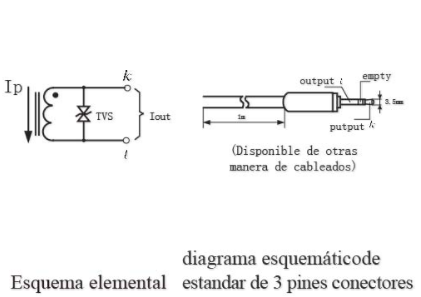
\includegraphics[scale=1]{imagenes/esquemapinza.png}
	\caption[YHDC.]{YHDC. Fuente: \cite{sensorcorriente}}
	\label{fig:pinza}
\end{figure}

\subsection{Módulo conversor analógico digital}
El propio ESP8266 pueda realizar una conversión de una señal analógica a una digital mediante el PIN A0 con una resolución de 10 bits.

Sin embargo si utilizamos el conversor analógico digital ADS 1115 conseguiremos una resolución de 16 bits. Además utilizando la biblioteca Adafruit\textunderscore ADS1015 \cite{adafruitbib} en concreto la función \textit{readADC\textunderscore Differential\textunderscore 0\textunderscore 1()} la cuál nos permite conocer la diferencia de voltaje entre el pin 0 y el pin 1 del ADS esto hace posible que no sea necesario el uso de dos resistencias en paralelo "bias resistor" . Para llevar a cabo nuestro esquema eléctrico tendremos que hacer uso de los pines VDD y GND los cuales alimentaremos a 3,3 V, los pines SCL y SDA para conectarlo al ESP8266 haciendo uso de la conexión I2C y los pines A0 y A1.

Las ventajas que nos ofrece este conversor analógico digital son:

\begin{itemize}
	\item Nos permite tener más precisión.
	\item Conexión I2C con la placa ESP8266.
	\item Elimina la necesidad de incorporar al circuito dos resistencias adicionales.
\end{itemize}


\begin{figure}[H]
	\centering
	\includegraphics[scale=0.6]{imagenes/ads1115.png}
	\caption[ADS1115.]{ADS1115. Fuente: \cite{adsfoto}}
	\label{fig:ads}
\end{figure}
\subsection{Módulo pantalla}

Como se especificó en el capítulo 2 de objetivos, el módulo de la pantalla corresponde a un objetivo opcional que finalmente se ha decidido incluir en el proyecto final.

A parte de ver la información detallada sobre los consumos en la web puede ser interesante para el usuario disponer de la información de forma inmediata y cómoda mediante una pantalla integrada en el propio dispositivo.

Debido a su bajo precio y que muchas de las soluciones para la medición de consumos eléctricos existentes en el mercado como se vio en el apartado 1.2 disponen se decidió que sería una buena idea incluirla en el diseño. Si la persona que desee realizar este proyecto no ve necesaria la utilización de esta pantalla se podría quitar sin ningún tipo de problema teniendo de esta manera la misma versión del dispositivo con las mismas funcionalidades pero sin la pantalla. 

Se trata de una pantalla LCD de 16x02 adquirida con un adaptador I2C directamente soldado a los pines que facilita de esta forma la conexión con el ESP8266. Gracias a la conexión I2C podemos conectar sin ningún tipo de problema a los puertos D1 y D2 de nuestro ESP8266 (puertos por defecto para la comunicación I2C en el ESP8266) especificando con que puerto queremos comunicarnos no tendremos ningún tipo de problema a la hora de que tanto el conversor de señal analógico digital (ADS1115) y el LCD compartan la conexión con los puertos D1 y D2.

\begin{figure}[H]
	\centering
	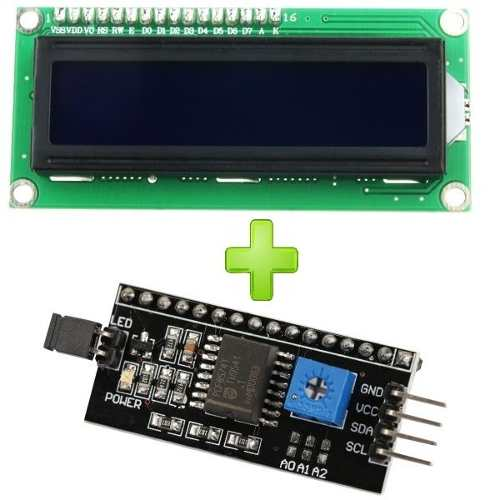
\includegraphics[scale=0.5]{imagenes/lcdi2c.jpg}
	\caption{LCD 16x02 y módulo I2C}
	\label{fig:lcdi2c}
\end{figure}

\section{Coste unitario}
Los precios mostrados a continuación (\ref{tabla:precios}) pueden variar en función de la tienda donde se adquieran los productos además pueden variar su precio a la alza o a la baja con el paso del tiempo. No están reflejados los gastos de envío de los productos ya que varían mucho en función de la web donde se adquieran.

Cabe destacar que los precios de algunos de los productos que aparecen en la tabla como puede ser la PCB están calculados restando el precio de la parte utilizada para llevar a cabo el proyecto al precio de la PCB completa.


\begin{table}[H]
	\begin{center}
		\begin{tabular}{|l|l|}
			\hline
			Producto & Precio \\
			\hline \hline
			NodeMcu ESP8266 CP2102 & \EUR{5.54} \\ \hline
			YHDC Non-Invasive AC Current Sensor [100A/30A] & \EUR{5.41} \\ \hline
			ADS1115 16bits ADC+PGA  & \EUR{2.45} \\ \hline
			Pantalla LCD 16x02 (Opcional)  & \EUR{3.49} \\ \hline
			40x cable macho macho  & \EUR{1.80} \\ \hline
			Estaño  & \EUR{0.40} \\ \hline
			Tira pines macho  & \EUR{1} \\ \hline
			Tira pines hembra  & \EUR{3} \\ \hline
			Trozo de placa experimental prototipo (PCB) & \EUR{2} \\ \hline
			Resistencias, jack hembra, conector entrada alimentación & \EUR{4} \\ \hline
			Tornillos, tuercas & \EUR{0.50} \\ \hline
			\textbf{Total} & \textbf{\EUR{29.59}} \\ \hline
			\textbf{Total sin Pantalla LCD } & \textbf{\EUR{26.10}} \\ \hline
		\end{tabular}
		\caption{Listado de precios.}
		\label{tabla:precios}
	\end{center}
\end{table}

\section{Prototipos}

Todos los diseños de estos prototipos se han realizado con el programa Fritzing antes de llevar a cabo pruebas en la protoboard. Todos estos prototipos se han montado en una protoboard para ahorrarnos de esta forma tener que soldar y gastar más material cada vez que se quisiera probar un nuevo diseño.

En este apartado se detallan las mejoras y fallos de cada uno de los 4 diseños que se analizaron para la construcción de este proyecto:

\begin{itemize}
	\item \textbf{Prototipo 1: } Se trata de la versión inicial con la que comenzó este proyecto. Es un diseño básico que no cuenta ni con pantalla para mostrar información instantánea de los datos que está recogiendo el sensor en cada momento ni con una entrada para poder alimentarlo mediante un conector jack hembra de alimentación. La alimentación de este prototipo iba a través del micro-usb que incorpora la placa NodeMCU. 
	
	\begin{figure}[H]
		\centering
		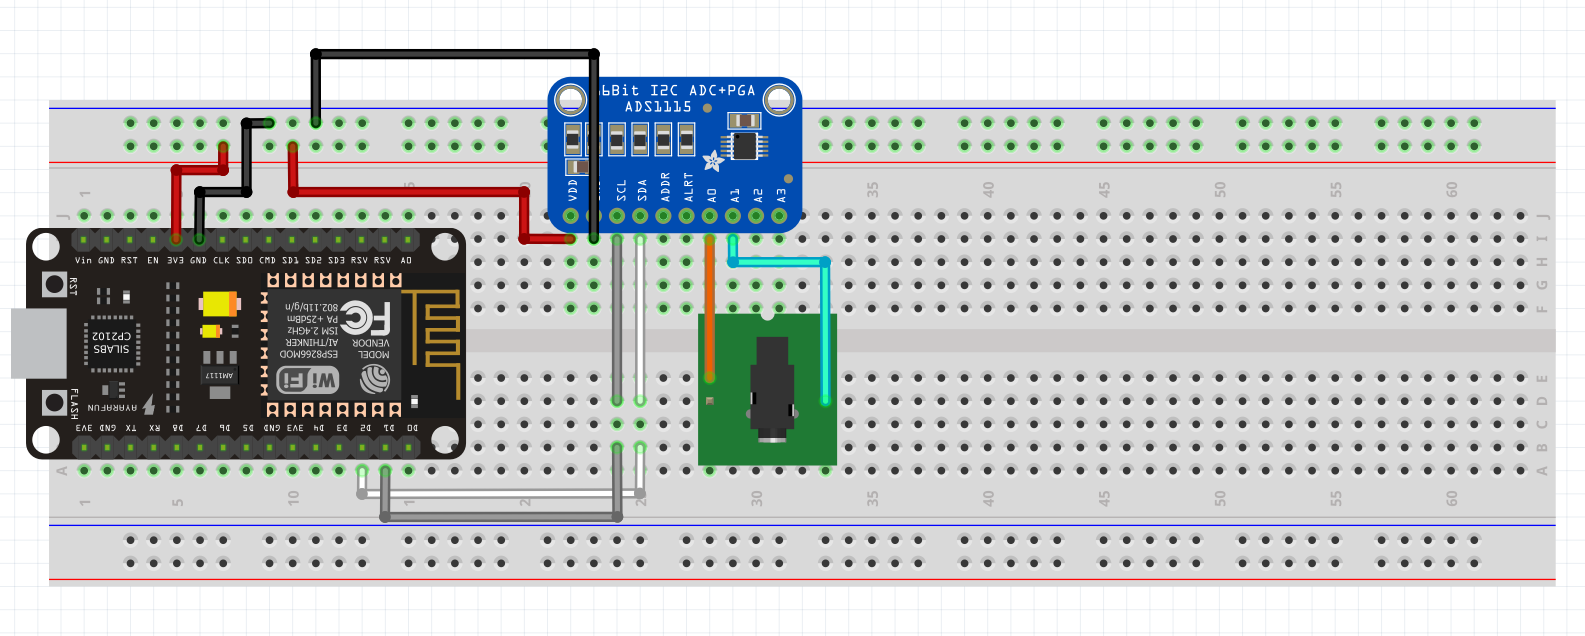
\includegraphics[scale=0.4]{imagenes/protoboardv1.png}
		\caption{Esquema v1}
		\label{fig:protoboardv1}
	\end{figure}

	\item \textbf{Prototipo 2: } Este prototipo incorpora un jack hembra de alimentación que permite alimentar el prototipo ya sea mediante el micro-usb propio de la placa o mediante un cargador de los que suelen usarse normalmente para alimentar otras placas como Arduino con una salida de 5V, lo que se pretendía con este prototipo era usar un único cargador con una salida de 5V para evitar que el usuario cogiera cualquier otro cargador de móvil o de algún otro dispositivo que disponga de una conexión micro usb ya que estos tienen una salida muy diferente los unos de los otros dependiendo de cuál sea el modelo de cargador y la empresa que fabrica el mismo.
	
	\begin{figure}[H]
		\centering
		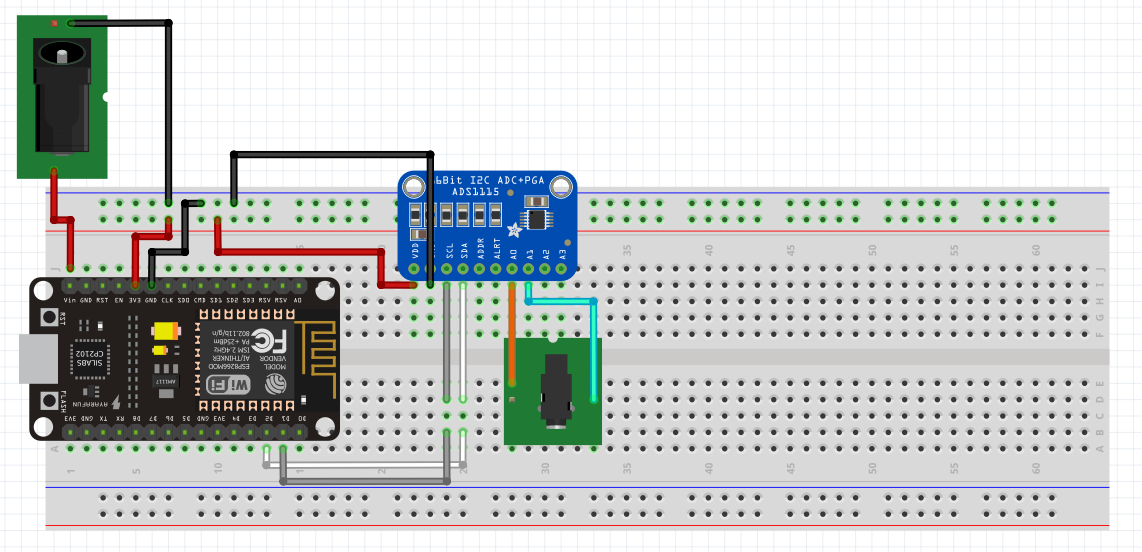
\includegraphics[scale=0.5]{imagenes/protoboardv2.png}
		\caption{Esquema v2}
		\label{fig:protoboardv2}
	\end{figure}
	
	
	\item \textbf{Prototipo 3: } En este diseño se incorpora el amplificador LM358 \cite{lm358} que intenta solucionar los malos resultados de los prototipos vistos anteriormente, pero realmente la solución a estos problemas se encontraban en la forma de poner el sensor de corriente ya que si el sensor rodea los dos cables la lectura no será correcta esta será cercana al 0 ya que los cables tienen corrientes opuestas, estas lecturas cercanas al 0 son el motivo principal por el que se intentó utilizar un amplificador de señal como solución al problema.
	
	\begin{figure}[H]
		\centering
		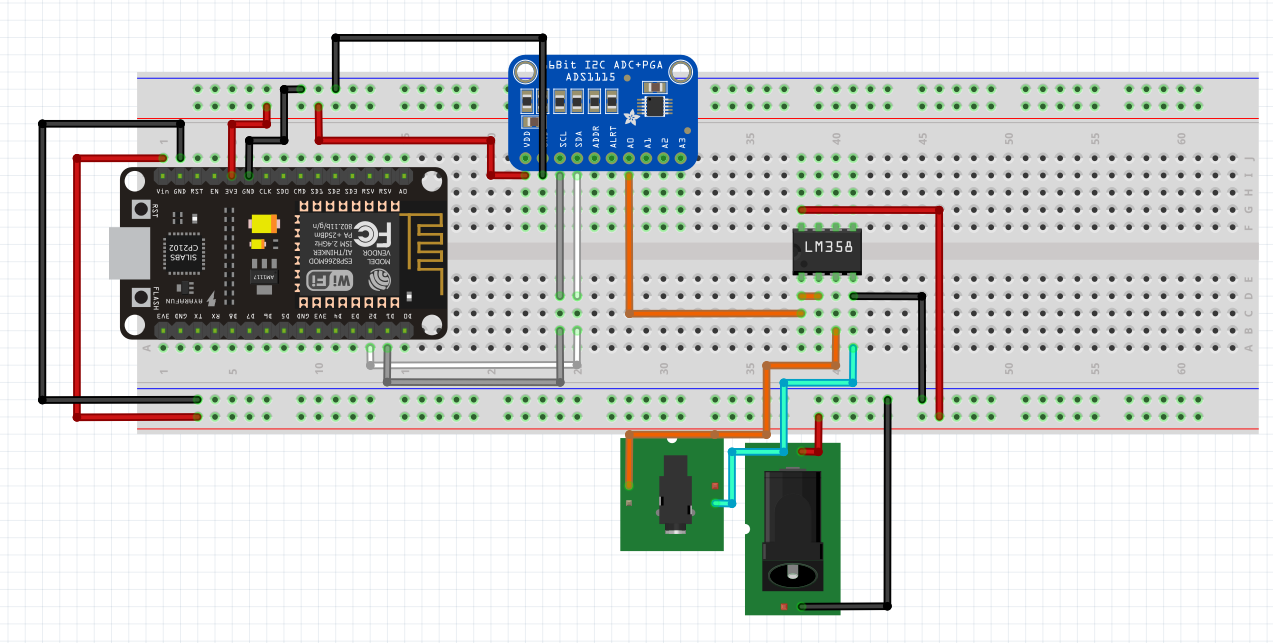
\includegraphics[scale=0.5]{imagenes/protoboardv3.png}
		\caption{Esquema v3}
		\label{fig:protoboardv3}
	\end{figure}
	
	\item \textbf{Prototipo 4: } Se trata de la versión final del proyecto la cuál incluye una pantalla LCD conectada mediante I2C que permite al usuario ver de una manera cómoda la información que está recogiendo en ese momento el sensor.
	
	\begin{figure}[H]
		\centering
		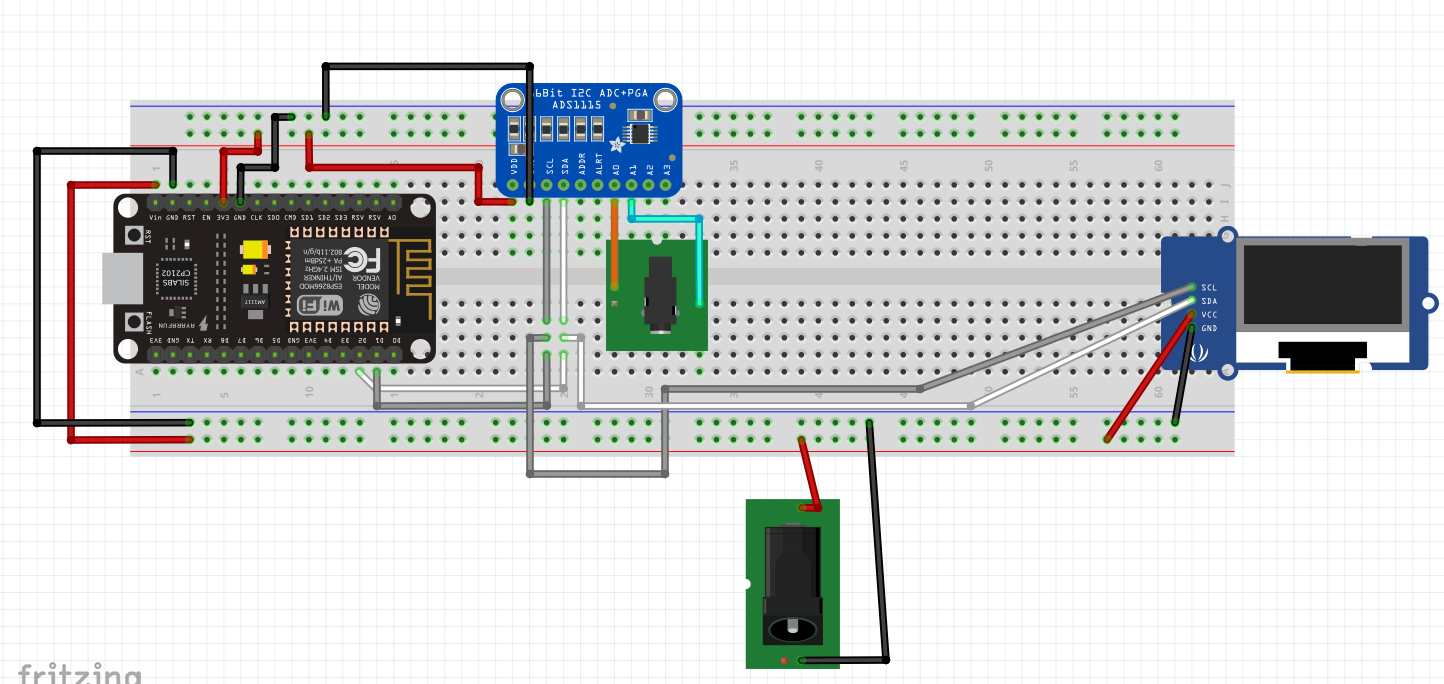
\includegraphics[scale=0.5]{imagenes/protoboardv4.png}
		\caption{Esquema v4}
		\label{fig:protoboardv4}
	\end{figure}
	
\end{itemize}

\section{Versiones finales}

En este apartado se verán los diseños de las dos versiones finales soldando pines hembra a una PCB para facilitar de esta forma el fácil reemplazo de los componentes en caso de que alguno de estos se estropeara o simplemente se quisiera retirar para darle otro uso sin que sufra ningún desperfecto a la hora de retirarlo.

El diseño para soldar las pistas de estaño en la PCB se ha realizado mediante el programa fritzing para asegurar que ninguna de estas pistas se toquen entre ellas provocando de esta forma un mal funcionamiento y al mismo tiempo nos aseguramos de que el tamaño de la placa esta utilizado de la mejor forma posible haciendo la placa lo más pequeña posible por si en un futuro se decidiera producir una gran cantidad de estas placas ahorrar costes de producción además de conseguir un dispositivo de menor tamaño.

\begin{itemize}
	\item \textbf{Versión 1 :} una vez que la persona interesada dio el visto bueno a este diseño (\ref{fig:pcbv1disenio}) realizado soldando pines hembra a una PCB para facilitar el cambio de componentes se pasa a realizar el primer modelo final soldado a una pcb como podemos ver en la imagen (\ref{fig:pcbv1}), observamos 8 conectores hembra donde van colocados los pines correspondientes a la alimentación y comunicación I2C de la pantalla LCD, los conectores para el jack del sensor de corriente y los conectores para conectar el jack de alimentación encargado de dar corriente al ESP8266.

	\begin{figure}[H]
		\centering
		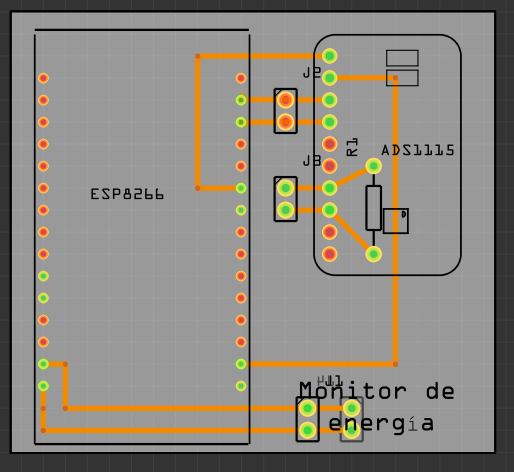
\includegraphics[scale=0.65]{imagenes/v1pcb.png}
		\caption{Esquema PCB versión 1}
		\label{fig:pcbv1disenio}
	\end{figure}

	\begin{figure}[H]
		\centering
		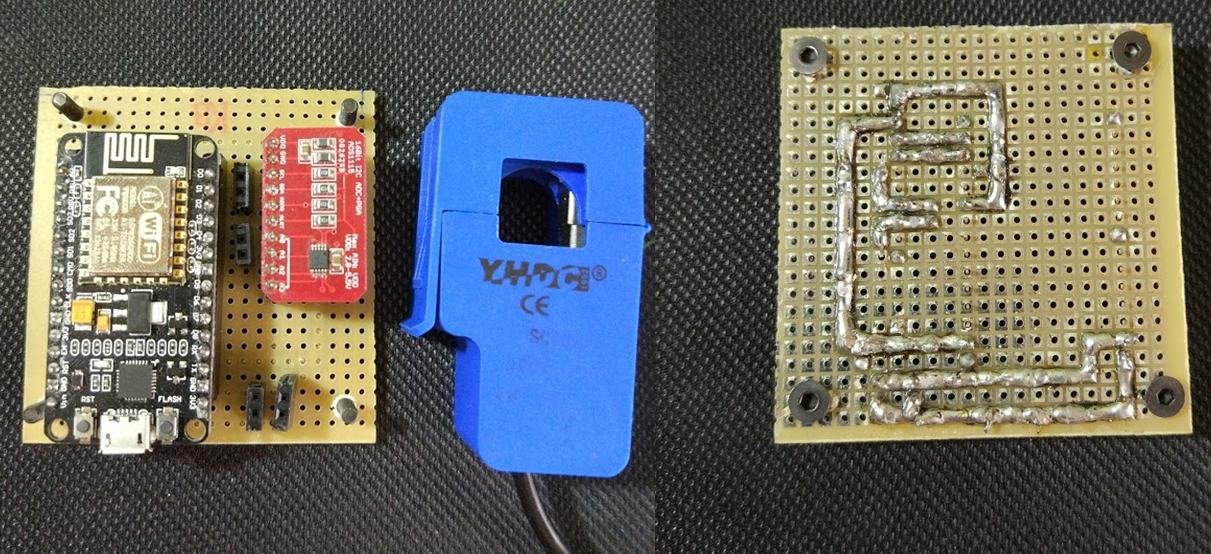
\includegraphics[scale=0.6]{imagenes/pcbv1.png}
		\caption{PCB soldada versión 1}
		\label{fig:pcbv1}
	\end{figure}

	\item \textbf{Versión 2 :} Con la idea de ahorrar espacio y hacer una caja de dimensiones algo más reducidas se estudió un nuevo diseño que permitiera tener uno de los lados de la placa con más espacio, con la idea de hacer la placa más larga que es algo poco importante ya que la caja de todas formas ha de tener el largo suficiente para poder alojar la pantalla LCD, pero un poco más estrecha pudiendo de esta manera colocar la pantalla LCD en uno de los laterales de la caja. Consiguiendo de esta forma que la tapa de la caja pese menos al no tener que soportar el peso de la pantalla LCD.
	
	\begin{figure}[H]
		\centering
		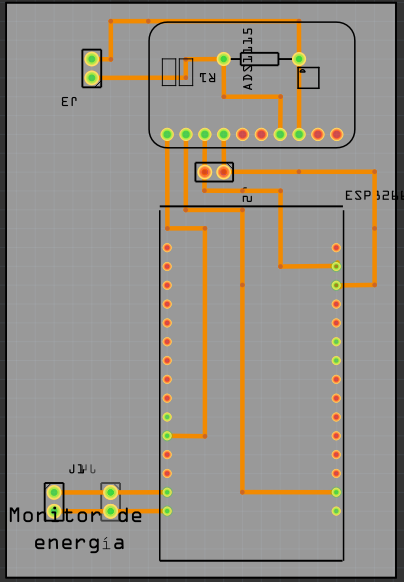
\includegraphics[scale=0.65]{imagenes/diseniopcbv2.png}
		\caption{Esquema PCB versión 2}
		\label{fig:pcbv2disenio}
	\end{figure}
	
	\begin{figure}[H]
		\centering
		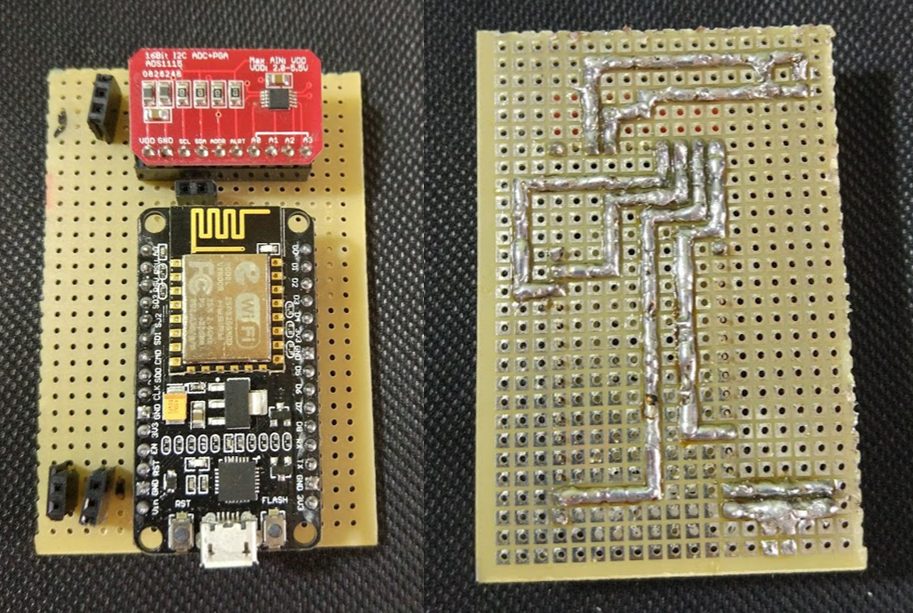
\includegraphics[scale=0.6]{imagenes/pcbv2.png}
		\caption{PCB soldada versión 2}
		\label{fig:pcbv2}
	\end{figure}

\end{itemize}



\section{Montaje de la caja}

Se ha utilizado una cortadora láser para construir las piezas necesarias para alojar la placa y los componentes necesarios en una caja.

Los primeros diseños de la caja están elaborados con DM ya que debido al bajo precio de este material nos permite realizar todas las pruebas que queramos y en caso de que alguna pieza no encaje o el resultado final no sea el esperado siempre podremos repetir esta pieza sin necesidad de desperdiciar un material de precio superior.

\begin{itemize}
	\item \textbf{Versión 1 :} En esta primera versión contamos con una caja básica que permite tener acceso tanto a la entrada micro usb de la placa ESP8266 por si fuera necesario cambiar el firmware de la misma, además de tener acceso a la entrada de jack del sensor de corriente y la entrada para la alimentación tal y como se puede apreciar en la imagen (\ref{fig:cajav1})
	
	\begin{figure}[H]
		\centering
		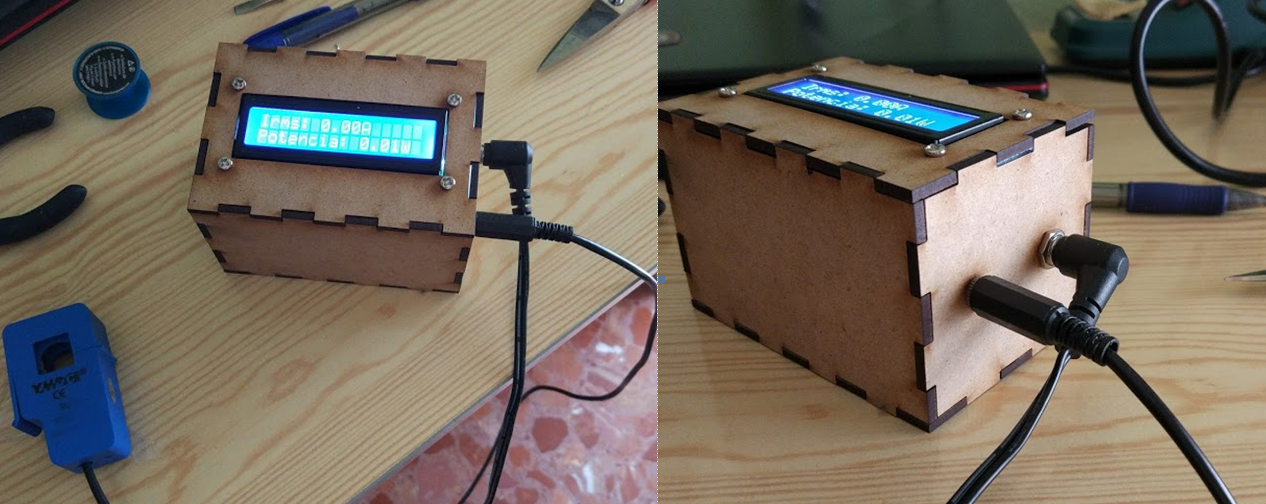
\includegraphics[scale=0.6]{imagenes/cajav1.png}
		\caption{Caja versión 1}
		\label{fig:cajav1}
	\end{figure}
	
	
	\item \textbf{Versión 2 :} En esta segunda versión se mejora la accesibilidad a los componentes que se encuentran en el interior de la caja introduciendo dos pestañas que actúan como bisagras (visibles en la imagen \ref{fig:cajav2}) sujetando la tapa de arriba de la caja la cuál incluye la pantalla haciendo posible de esta forma la apertura de la caja para cambiar cualquier elemento.
	
	\begin{figure}[H]
		\centering
		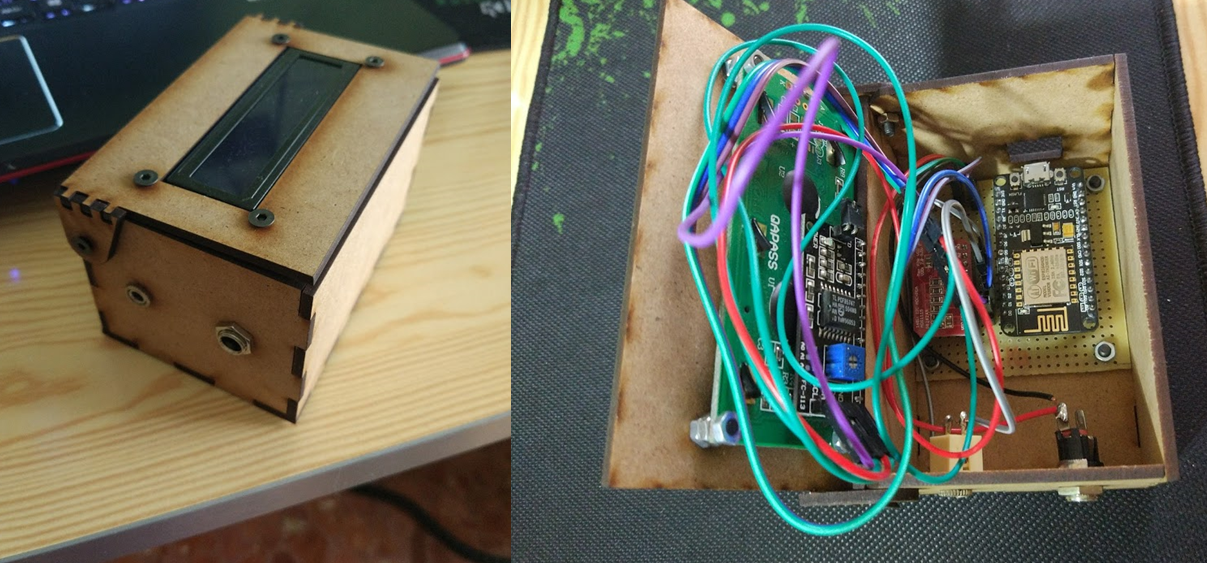
\includegraphics[scale=0.6]{imagenes/cajav2.png}
		\caption{Caja versión 2}
		\label{fig:cajav2}
	\end{figure}
	
\end{itemize}